\section{Pull payment (aka invoicing)} \label{sec:pull}

\begin{figure}[h!]
  \begin{sequencediagram}
    \newinst{payer}{\shortstack{Payer \\
      \\ 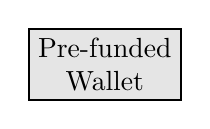
\begin{tikzpicture}
        \node [fill=gray!20,draw=black,thick,align=center] {Pre-funded \\ Wallet};
      \end{tikzpicture}
    }}
    \newinst[2]{exchange}{\shortstack{Taler (exchange) \\
       \\ \begin{tikzpicture}[shape aspect=.5]
        \tikzset{every node/.style={cylinder,shape border rotate=90, draw,fill=gray!25}}
        \node at (1.5,0) {\shortstack{{{\tiny Database}}}};
       \end{tikzpicture}
    }}
    \newinst[2]{payee}{\shortstack{Payee \\
      \\ 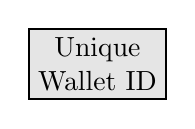
\begin{tikzpicture}
        \node [fill=gray!20,draw=black,thick,align=center] { Unique \\ Wallet ID};
      \end{tikzpicture}
    }}
    \postlevel
    \begin{callself}{payee}{Review pull payment fees}{}
    \end{callself}
    \mess[0]{payee}{{Create invoice (Wallet ID)}}{exchange}

    \mess[0]{exchange}{{Invoice ready}}{payee}
    \mess[0]{payee}{{Send invoice (e.g. via QR code)}}{payer}

    \begin{callself}{payer}{Review invoice}{}
    \end{callself}
    \mess[0]{payer}{{Make payment (Coins)}}{exchange}

    \begin{sdblock}{Domestic wallet?}{}
    \begin{callself}{exchange}{Figure~\ref{fig:proc:domestic}}{}
    \end{callself}
    \end{sdblock}
    \begin{sdblock}{KYC/AML required?}{}
    \begin{callself}{exchange}{Figures~\ref{fig:proc:kyc}, \ref{fig:proc:aml}}{}
    \end{callself}
    \end{sdblock}

    \mess[0]{exchange}{{Distribute digital cash}}{payee}

\end{sequencediagram}
  \caption{Interactions between wallets and Taler exchange
    in a pull payment.}
  \label{fig:int:pull}
\end{figure}

We do {\bf not} permit the payer to regain control over their funds, once the
payment was made they are locked {\em until} the payee passes the KYC/AML
checks.  We only do the AML/KYC process once the funds are locked at the
exchange. This ensures we know the actual transacted amounts (which may be
lower than the total amounts requested) and prevents risk-free probing
attacks.
